\title[P\&S 2026/2027]{Probability \& Statistics (Premaster MTPS)}
\subtitle[College 2]{College 2}  
\author{Dr. ir. D.A.M.P. Blom}
\institute[NLDA]{Nederlandse Defensie Academie}
\date{16 oktober 2026}
\begin{document}

\begin{frame}
    \maketitle
    % \begin{center}
    %     \includegraphics[width=3cm]{1_marine}
    %     \includegraphics[width=3cm]{1_luchtmacht}
    %     \includegraphics[width=3cm]{1_landmacht}
    % \end{center}
\end{frame}

%------------------------------------------------%	
\begin{frame}{Agenda}
    Vandaag: college van 9.20 tot 14.00 uur (daarna: inzage Calculus)
    \vfill
    \begin{itemize}
        \item 9.20 - 10.00 uur: recap van vorige les
        \item 10:15 - 11.00 uur: discrete en continue kansvariabelen
        \item 11.15 - 12.00 uur: normale verdeling en de centrale limietstelling
        \item 12.00 - 12.45 uur: lunchpauze
        \item 12.45 - 14.00 uur: gezamenlijke kansverdelingen
    \end{itemize}
    \vfill
    \textbf{Dit komt ruwweg overeen met de inhoud van learning tasks 4 t/m 10.}
\end{frame}

\begin{frame}{Kansexperiment}
    \textbf{Input:} \medskip

    \begin{itemize}
        \item Uitkomstenruimte $S$
        \item Onderliggende kansverdeling over $S$
    \end{itemize}\medskip

    \textbf{Experiment:} \medskip

    \begin{itemize}
        \item Lab-meting
        \item Afname van een enquête
        \item Simulatie
        \item $\ldots$
    \end{itemize}\medskip

    \textbf{Output:} \medskip

    \begin{itemize}
        \item Een trekking van exact één van de uitkomsten in de uitkomstenruimte
    \end{itemize}
\end{frame}

\begin{frame}{Gebeurtenissen}
    Een \concept{gebeurtenis} (\emph{event}) in een kansexperiment is een deelverzameling van de uitkomstenruimte ($E \subseteq S$):
    \begin{itemize}
        \item $A$: er wordt minstens één keer een drie gegooid met twee dobbelstenen.
        \[
            A = \set{(3,1), (3,2), (3,3), \ldots, (4, 3), (5, 3), (6, 3)}
        \]
        \item $B$: de som van twee dobbelsteenworpen is gelijk aan $7$:
        \[
            B = \set{(1,6), (2,5), (3,4), (4,3), (5,2), (6,1)}
        \]
    \end{itemize}
    Naast losse gebeurtenissen kunnen we ook kijken naar samenstellingen, zoals $A'$, $A \cup B$, $A \cap B$.
\end{frame}

\begin{frame}{Overzicht van rekenregels}
    \begin{itemize}[<+->]
        \item Complementregel (voor gebeurtenis $A$):
        \[
            P(A) = 1 - P(A').
        \]
        \item Algemene optelregel (voor gebeurtenissen $A$ en $B$):
        \[
            P(A \cup B) = P(A) + P(B) - P(A \cap B).
        \]
        \item Conditionele kansen:
        \[
            P(A | B) = \frac{P(A \cap B)}{P(B)}
        \]
        \item Bayes' regel:
        \[
            P(A | B) = \frac{P(B | A) \cdot P(A)}{P(B)}
        \] 
        \item Onafhankelijkheid:
        \[
            P(A \cap B) = P(A) \cdot P(B | A) = P(A) \cdot P(B)
        \]
    \end{itemize}
\end{frame}

\begin{frame}{Oefening: faalgedrag van componenten}
    Wat is de kans dat het gehele circuit blijft functioneren?
    \begin{center}
        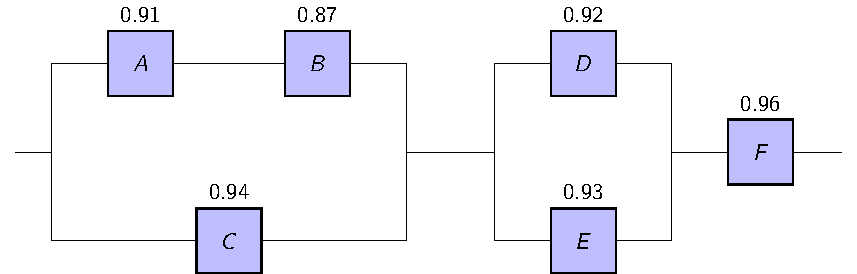
\includegraphics[width=0.9\textwidth]{../tikz/2_example_circuit.pdf}%
    \end{center}
\end{frame}

\begin{frame}{Kansvariabelen}
    Er zijn twee soorten kansvariabelen: \concept{discrete} en \concept{continue kansvariabelen}:
    \vfill
    \begin{center}
        \begin{tabular}{lll}
            \toprule
                \textbf{Discrete kansvariabelen} & \textbf{Continue kansvariabelen} \\
            \midrule
                Losse, afzonderlijke getallen & Interval van getallen \\
                Tellen of categoriseren       & Meten \\
            \bottomrule       
        \end{tabular}
    \end{center}
\end{frame}

\begin{frame}{Discrete kansvariabelen}
    Een \concept{discrete kansvariabele} is een kansvariabele met een \emph{eindige} of \emph{aftelbaar oneindige} uitkomstenruimte van numerieke waarden.
    \vfill
    \textbf{Voorbeelden:}
    \begin{itemize}
        \item Aantal keer dat een doel wordt geraakt bij $10$ schoten ($0, 1, \ldots, 10$).
        \item Aantal door EOD geruimde WO2-bommen in Nederland in een week ($0, 1, \ldots$).
        \item Aantal pogingen totdat een cyberaanval slaagt ($1, 2, \ldots$).
        \item Al dan niet detecteren van een vijandelijke drone ($0, 1$).
    \end{itemize}

\end{frame}

\begin{frame}\frametitle{Samenvatting: discrete kansvariabelen}

    {\scriptsize
    \begin{center}
        \begin{tabular}{m{0.3\textwidth}m{0.6\textwidth}}
            \toprule
                & \textbf{Discreet} \\
            \midrule
                \uncover<+->{\textbf{Uitkomstenruimte $S$:}  & eindig / aftelbaar oneindig} \\ \midrule
                \uncover<+->{\textbf{Kansbegrip:}        & kansmassafunctie $f(x) = P(X = x)$: \begin{itemize} \item $f(x) \geq 0$ voor iedere uitkomst $x$ 
                    \item $\sum_{x \in S} f(x) = 1$ \end{itemize}} \\ \midrule
                \uncover<+->{\textbf{Verdelingsfunctie (CDF):} & $F(x) = P(X \leq x) = \sum_{y \leq x} f(y)$
                \begin{itemize} \item $F$ is monotoon niet-dalend
                                \item $\lim_{x \to \infty} F(x) = 0$ en $\lim_{x \to \infty} F(x) = 1$
                            \end{itemize}} \\ \midrule
                \uncover<+->{\textbf{Verwachtingswaarde:} & $E(X) = \sum_{x \in S} x \cdot f(x)$} \\ \midrule
                \uncover<+->{\textbf{Variantie:} & $\Var{X} = \sum_{x \in S} \left(x - E(X)\right)^2 \cdot f(x)$} \\ \midrule
                \uncover<+->{\textbf{Standaardafwijking:} & $\sigma(X) = \sqrt{\Var{X}}$} \\                 
            \bottomrule
        \end{tabular}   
    \end{center}
    }
\end{frame}

\begin{frame}{Continue kansvariabelen}
    Een \concept{continue kansvariabele} is een kansvariabele met een \emph{oneindige} uitkomstenruimte van numerieke waarden.
    \vfill
    \textbf{Voorbeelden:}
    \begin{itemize}
        \item Reactietijd van een F-35 vlieger.
        \item Afgelegen afstand tijdens een coopertest.
        \item Dikte van een pantserplaat bij een infanterievoertuig.
        \item Waterdiepte bij een amfibische landingslocatie.
    \end{itemize}
    \vfill In plaats van losse, onderscheidbare \emph{discrete} waarden, hebben we hier te maken met een \emph{continu} spectrum van mogelijke uitkomsten.
\end{frame}

\begin{frame}{Voorbeeld: inslaglocatie van mortiergranaten}
    Bij een schietoefening met een mortierpeloton wordt gekeken hoe precies een doel op 3 km afstand kan worden beschoten. 
    Bij een test met 81mm mortiergranaten wordt de afstand gemeten van het inslagpunt tot het beoogde doel.
    \vfill
    \textbf{Wat is de kans dat een willekeurige mortiergranaat op precies $56.12843926$ meter van het doel inslaat?}\\[1ex]
    \pause

    \emph{Die kans is nul!}
    \pause\vfill

    Toch weten we van kansexperimenten dat er uiteindelijk een uitkomst gerealiseerd wordt.
    In de continue wereld betekent kans $0$ dus niet hetzelfde als \enquote{onmogelijk!}.
\end{frame}

\begin{frame}\frametitle{Kansen bij continue kansvariabelen}
    Om intuïtie te krijgen, helpt het om terug te werken naar de discrete wereld:
    \begin{itemize}\setlength\itemsep{2em}
        \item De uitkomstenruimte van ons voorbeeld is $S = \set{x \mid x \geq 0}$.
        \item In plaats van kijken naar losse uitkomsten (zoals $56.12843926$ meter), gaan we $S$ opdelen in \emph{discrete klassen}, bijv.:
        \[
            [0, 1), [1, 2), \ldots
        \] 
        \item Als we data verzamelen uit het kansexperiment (mortiergranaten afvuren en afstand meten), kunnen we een \concept{histogram} maken van de discrete klassen.
    \end{itemize}
\end{frame}

\begin{frame}{Voorbeeld: inslaglocatie van mortiergranaten}
    \begin{center}
        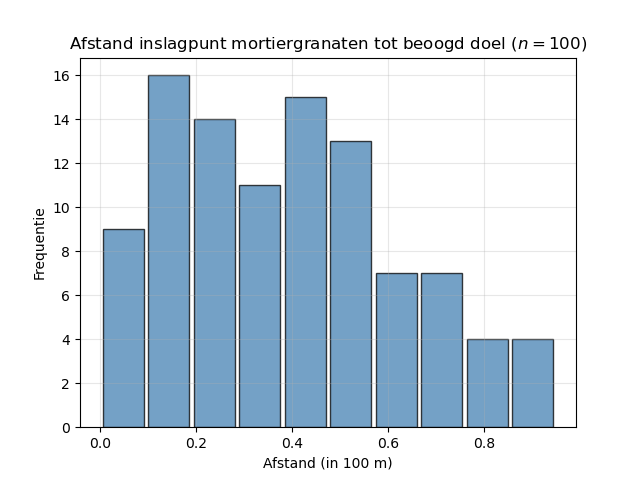
\includegraphics[width=0.85\textwidth]{../figures/2_mortar_grenades_hist_n=100_bins=10.png}
    \end{center}
\end{frame}

\begin{frame}{Voorbeeld: inslaglocatie van mortiergranaten}
    Zodra je het aantal waarnemingen vergroot en het aantal bins (klassen):
    \begin{center}
        \begin{tabular}{cc}
            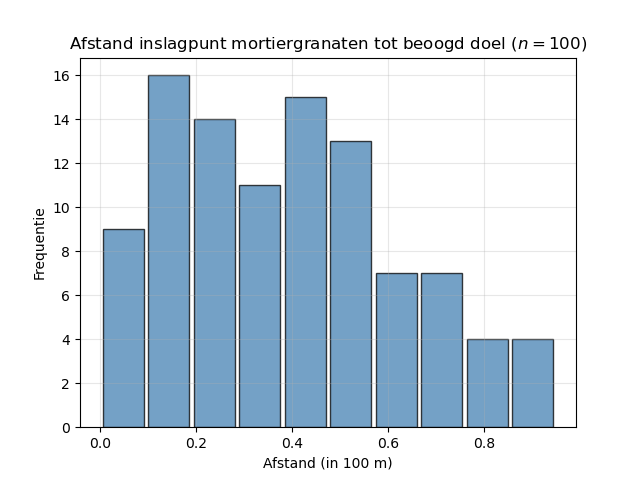
\includegraphics[height=0.4\textheight]{../figures/2_mortar_grenades_hist_n=100_bins=10.png} & 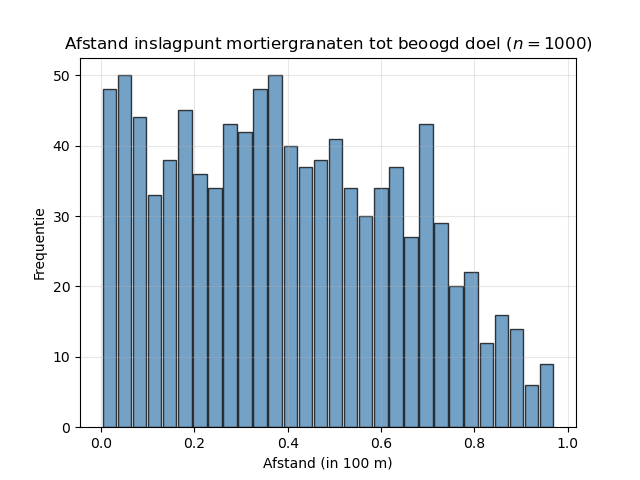
\includegraphics[height=0.4\textheight]{../figures/2_mortar_grenades_hist_n=1000_bins=30.png} \\
            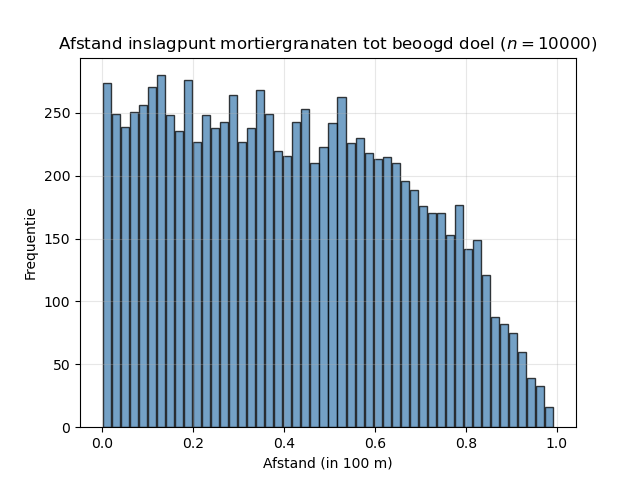
\includegraphics[height=0.4\textheight]{../figures/2_mortar_grenades_hist_n=10000_bins=50.png} & 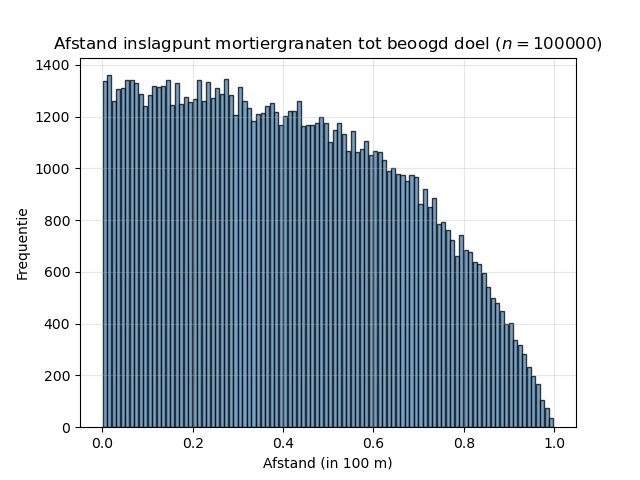
\includegraphics[height=0.4\textheight]{../figures/2_mortar_grenades_hist_n=100000_bins=100.png} \\
        \end{tabular}
    \end{center}
\end{frame}

\begin{frame}{Voorbeeld: inslaglocatie van mortiergranaten}
    Als het aantal waarnemingen heel groot is, lijkt de histogram steeds beter op een \enquote{vloeiende lijn}.
    \begin{center}
        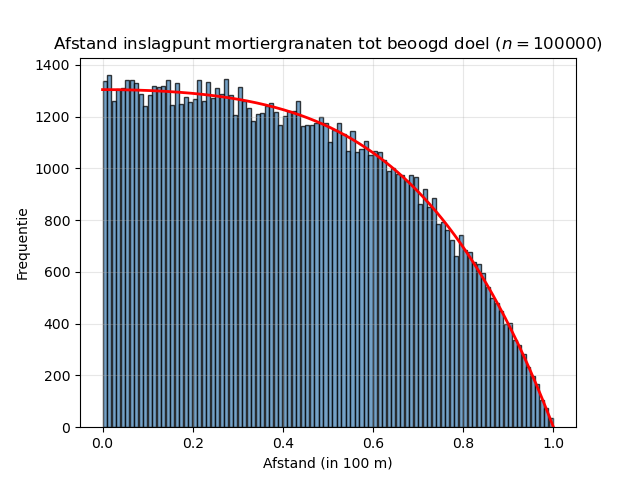
\includegraphics[height=0.75\textheight]{../figures/2_mortar_grenades_hist_n=100000_bins=100_with_pdf.png}
    \end{center}
\end{frame}

\begin{frame}{Kansdichtheidsfunctie}
    Deze vloeiende lijn noemen we de \concept{kansdichtheidsfunctie} $f(x)$ van een continue kansvariabele $X$.
    De hoogte van deze functie wordt geschaald zodat: 
    \begin{itemize}[<+->]
        \item De oppervlakte onder $f(x)$ is gelijk aan $1$:
        \[
            \int_{x} f(x) \dx = 1
        \]
        \item De kansdichtheidsfunctie $f(x)$ is overal niet-negatief:
        \[
            f(x) \geq 0 \text{ voor alle } x
        \]
    \end{itemize}

    \pause
    \textbf{Let op: } $f(x)$ is \underline{niet} hetzelfde als $P(X = x)$, want $P(X=x) = 0$!
    
    We kunnen alleen kansen uitrekenen op een \emph{interval} van uitkomsten:
    \[
        P(a \leq X \leq b) = \int_a^b f(x) \dx
    \]
\end{frame}

\begin{frame}{Voorbeeld: inslagpunt van mortiergranaten}
    Bij een schietoefening met een mortierpeloton wordt gekeken hoe precies een doel op 3 km afstand kan worden beschoten. 
    Bij een test met 81mm mortiergranaten wordt de afstand gemeten van het inslagpunt tot het beoogde doel.

    De afstand $X$ (in honderden meters) volgt de volgende kansdichtheidsfunctie:
    \[
        f(x) = 
        \begin{cases} 
            c \cdot (4 - x^2 - 3x^4), & \text{ voor } -1 \leq x \leq 1, \\
            0,                        & \text{ anders.}
        \end{cases}
    \]

    \begin{enumerate}[label=(\alph*)]
        \item Bereken $c$ zodanig dat $f(x)$ een goed gedefinieerde kansdichtheidsfunctie is.
        \item Wat is de kans dat de mortier binnen $30$ meter van het beoogde doel inslaat?
    \end{enumerate}
\end{frame}

\begin{frame}{Bereken $c$ zodanig dat $f(x)$ een goed gedefinieerde kansdichtheidsfunctie is.}
    Een goed gedefinieerde kansdichtheidsfunctie $f(x)$ voldoet aan twee eisen:
    \begin{itemize}
        \item De oppervlakte onder $f$ is gelijk aan $1$:
        \begin{align*}
            1 = \int_x f(x) \dx &= \int_{x=-1}^1 c \cdot (4 - x^2 - 3x^4) \dx \\
                                &= c \cdot \int_{x=-1}^1 (4 - x^2 - 3x^4) \dx \\
                                &= c \cdot [4x - \frac{1}{3}x^3 - \frac{3}{5}x^5|_{x=-1}^1 \\
                                &= c \cdot ((4-\frac{1}{3}-\frac{3}{5})-(-4+\frac{1}{3}+\frac{3}{5})) \\
                                &= c \cdot \frac{92}{15}
        \end{align*}
        Hieruit volgt dat $c = \frac{15}{92}$.
        \item $f(x) \geq 0$ voor alle $x$:
        
        Merk op dat op het interval $[-1, 1]$, de term $4 - x^2 - 3x^4$ altijd groter dan of gelijk aan $0$ is. 
        Als je dit vermenigvuldigt met $c = \frac{15}{92}$ blijft dat zo, oftewel $f(x) \geq 0$ voor alle $x$.
    \end{itemize}
\end{frame}

\end{document}